\documentclass[12pt,oneside]{gsbook}
\usepackage{greensocs}

\usepackage{xspace}
\usepackage{fancyvrb}

\newcommand{\master}{{\em System Initiator}\xspace}
\newcommand{\masters}{{\em System Initiators}\xspace}
\newcommand{\slave}{{\em System Target}\xspace}
\newcommand{\slaves}{{\em System Targets}\xspace}
\newcommand{\router}{{\em System Interconnect}\xspace}
\newcommand{\routers}{{\em System Interconnects}\xspace}

\newcommand{\atom}{{\em Phase}\xspace}
\newcommand{\atoms}{{\em Phases}\xspace}
\newcommand{\quark}{{\em Attribute}\xspace}
\newcommand{\quarks}{{\em Attributes}\xspace}

\def\example#1{\begin{center}\colorbox{lightgrey}{\begin{tabular}{|p{0.6\paperwidth}|}\hline\\#1\\ \\ \hline\end{tabular}}\end{center}}

\newsavebox{\examplebox}
\newenvironment{exampleenv}{\begin{lrbox}{\examplebox}\begin{minipage}{0.6\paperwidth}}{\end{minipage}\end{lrbox}\example{\usebox{\examplebox}}}
\newcommand{\tick}{$\sqrt{}$}

\author{Copyright GreenSocs Ltd 2006}
\title{GreenBus User Manual}

\begin{document}
\maketitle
\tableofcontents


\chapter{Terminology}
\label{TERMS}
In order to discuss ``Transaction Level Modeling'' several terms are
needed,  what a transaction is, and between who it is
exchanged.

\begin{figure}[htbp]
        \centering
        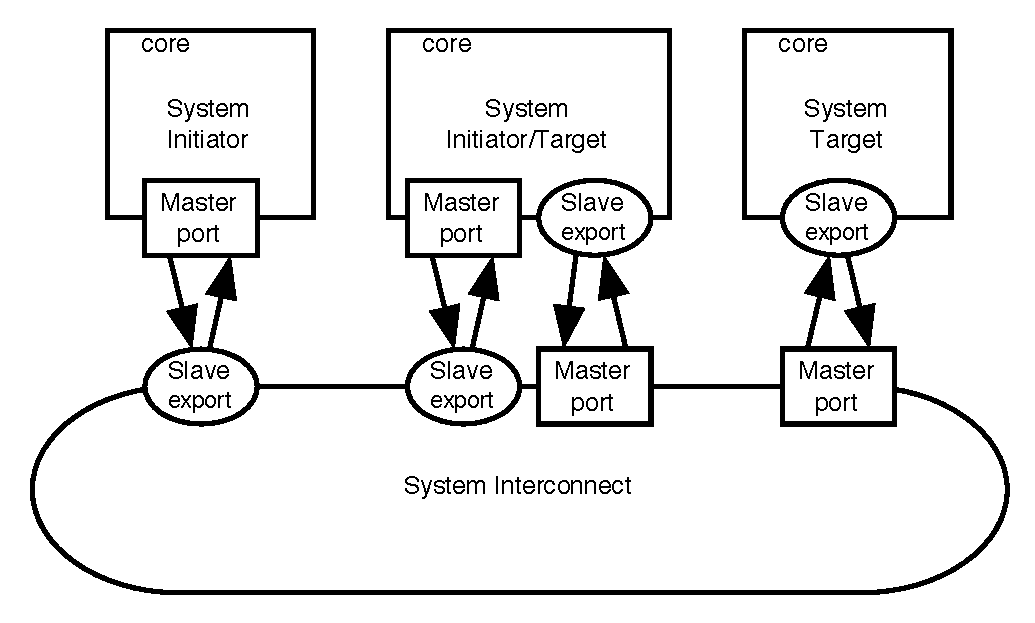
\includegraphics{names.eps}
        \caption{Naming convention}
        \label{fig:naming}
\end{figure}


Within a system, we specify three types of object (as shown in figure~\ref{fig:naming}):
\begin{description}
\item [\masters] These objects are responsible for starting a
message.
\item [\slaves] These objects will receive and respond to a
message.
\item [\router] These objects pass the message between
\masters and \slaves
\end{description}

A transaction is a message passed between a \master, via
none, one or more \routers to a \slave, who may (or
may not) reply back via the \router to the \master
. The entire communication between \master and
\slave we call a Transaction.

More formally, within SystemC, a \master has (at least) a master
sc\_port, a \slave has a slave sc\_export, and a \router
has a slave sc\_export and a master sc\_port. We further constrain
these terms : a \master initiates (and allocates memory for) a
transaction, while a \slave responds to transaction. 

A transaction is broken down into a Request and a Response. The
Request goes between the \master and the \slave, the
Response goes between the \slave and the \master.

Request and Response structures can be further broken down into the
control and data items that they contain. We call these \quarks.
A \quark can be the data being passed between the \master
and the \slave, or the address of the \slave, or the control information
indicating that the \master wishes to read data from the \slave, etc.

The information contained within a transaction takes some time to
transmit. In fact many transactions may be active at any one moment in
time, and it will be the job of the \router to arbitrate between
them. In order for this to happen, transactions are split over time
into ``chunks'' of data.  We call these \atoms. Once active on a
\router, in principle a \atom can not be interrupted. 

Most busses use 3 types of \atom, 
\begin{itemize}
\item A Request \atom which often covers the time taken to transmit
the  information in the ``Request'' structure mentioned above.
\item  A ``Data Handshake'' \atom which often covers the time taken to
transmit a small amount of data. For transactions containing large data items,
there will typically be multiple Data Handshake \atoms, each containing
a small proportion of the data.
\item A ``Response'' \atom which typically covers the time taken to
transmit the information in the ``Response'' structure above (though
may not have the whole response data in it)
\end{itemize}

There are therefore, typically, 6  interesting ``time points'', the
start and end of each of these \atoms (and 2 more for each data
handshake \atom used).

{\bf Notice: Transactions pass between \masters and \slaves, but
\atoms indicate the state of that communication between any pair of
\master, \router or \slave in the communication path}

\section{Abstraction levels}

We are now in a position to more formally define ``abstraction
levels''. They are levels at which different aspects of a transaction
are of interest.

\begin{tabular}{l|c|p{6cm}}
{\bf Some Names}&{Unit of interest}&{User}\\
\hline
pv & Transaction Data & Programmers Model for many Software Tasks \\
pv, av, pvt &  \atoms & System Engineers Model,Gives relatively good timing accuracy\\
vv, cc, pvt & \quark & Detail Designers Model (either for specific S/W or H/W design/verification)\\
RTL & 	Signal &  RTL Engineers Model\\
\end{tabular}

While the naming conventions different people have used are
overlapping and confusing, and the use models are diverse, the unit of
interest is a clear differentiator for model types.

\chapter{Goals of GreenBus}

The goals for GreenBus are :
\begin{description}
\item[Inter-operability] To have a simple API between models, with
defined  data structures and semantics such that interoperability can
be guaranteed.

\item [Safety] Automatic memory management for data structures, and
event semantics between models. The event semantics between the models
is especially important to guarantee that the interfaces behave in an
predictable and expected manor.

\item [Speed] Although speed is listed last, but it is still of utmost
importance. The goal is to minimize the amount
of data coping required. Only the minimum of events must be used, and
the model style should encourage the use of event sensitive methods
rather than ``{\tt wait()}'' calls.
\end{description}

\section{Interoperability Interface}
\label{INTEROP}

In July 2007, GreenSocs defined a very simply ``interoperability interface''
and proposed it  to the TLM WG for inclusion in the TLM 2.0
standard.

This interface is extremely simple. It consists of 2 pairs of
port/exports.

\begin{exampleenv}
\begin{Verbatim}[ numbers=left,fontsize=\small]
  template <class PV, class PVT>
  class tlm_port
  {
public:

    sc_port<tlm_b_if<PV> > b_out;
    sc_export<tlm_b_if<PV> > b_in;

    sc_port<tlm_peq_if<PVT> > out;
    sc_export<tlm_peq_if<PVT> > in;

   ....

}
\end{Verbatim}
\end{exampleenv}


\subsection{Blocking Interface}

The first pair implements the {\tt tlm\_b\_if} which in itself is very
simple:

\begin{exampleenv}
\begin{Verbatim}[ numbers=left,fontsize=\small]
  template <class TRANSACTION>
  class tlm_b_if : public virtual sc_interface
  {
  public:
    virtual void b_transact( TRANSACTION) = 0;
  };
\end{Verbatim}
\end{exampleenv}

The {\tt b\_transact} function must be implemented by the sc\_export, and will
be expected by the sc\_port. The function is blocking (in  SystemC
this means the function MAY call ``{\tt wait()}'', and time may elapse until
the function returns). When it does return, the transaction will have been
completed. If there is return data it will be available (though, of
course, there may have been an error, so the data may not be valid).

There is a useful use for {\tt wait()} inside a programmers view model,
that would otherwise be totally un-timed. This is to allow models to
``yield'' to other threads within the system. These are often called
synchronization points.

All that remains is to define the transaction type itself. To ensure
that the types are similar, the boost library can be used. These asserts
can be places in the tlm\_port class.


\begin{exampleenv}
\begin{Verbatim}[ numbers=left,fontsize=\small]
  template <class PV, class PVT>
  class tlm_port
  {
private:
    
    BOOST_STATIC_ASSERT(( boost::is_base_of<
	boost::shared_ptr<TransactionBase>, PV>::value ));
   ....

  }
\end{Verbatim}
\end{exampleenv}


A transaction is expected to inherit from TransactioBase, and use ONLY
the \quarks defined in the {\tt Attributes.h} class. These will be
examined in Chapter~\ref{PROTOCOL}.

The interoperability interface
does not define the data payload that is to be used, but an example is
given, that covers most bus fabrics. This is called the ``generic''
protocol. Inheriting from the generic protocol will greatly increase
interoperability.


\subsection{Non Blocking Interface}
The second pair implements the {\tt tlm\_peq\_if} which is also
simple. (PEQ stands for ``Payload Event Queue'' and is name this way
to reflect the semantic expectations on the function calls).


\begin{exampleenv}
\begin{Verbatim}[ numbers=left,fontsize=\small]
  template <typename PAYLOAD>
  class tlm_peq_if
  {
public:
    
    virtual void write (PAYLOAD)=0;
    virtual void write (PAYLOAD, const sc_time& when)=0;
    virtual void write (PAYLOAD, double when, sc_time_unit base)=0;
  };
\end{Verbatim}
\end{exampleenv}

The write function has the same semantics as the ``notify'' function
call for a normal {\tt sc\_event}. The {\tt PAYLOAD} must be delivered
to the model at the time indicated.

The means by which the data {\tt PAYLOAD} is delivered to the model is {\em
NOT} defined in the interoperability interface, as it is the concern
of the implementation of the interoperability layer. The user interface to
the GreenBus implementation will be examined in Chapter~\ref{USER}.

The implementation need not use events, but it must arrange (somehow)
to deliver the {\tt PAYLOADS} to the model at the time indicated.

The first form of the {\tt write} method (line 6) takes no time
argument. This form is the  equivalent of a {\tt notify} function with
no time, it should
only deliver its {\tt PAYLOAD} once the current method yields - but
within the same simulation delta. More
formally, the semantic that must be guaranteed is that the caller of
the {\tt write} function must not be able to detect a change in the
system until after it yields (by itself calling wait, or returning from
an event sensitive method).

Finally, if multiple {\tt PAYLOADS} are scheduled to arrive at the same
time, then they {\em must} all be delivered in the same delta. 

The timing interface payload is a pair: the transaction data (as
defined in the previous section) and a ``timing state''. The ``timing
state'' is used to determine which state the current {\tt PAYLOAD}
delivery  is moving the communication state machine into. This can be
as simple as an integer value.

The interoperability interface does not define the state machine, but again the
generic protocol (see Chapter~\ref{PROTOCOL}) does. Using the generic
protocol will greatly increase interoperability.

The following code can be included in the tlm\_port to ensure that the PVT
{\tt PAYLOAD} is of the correct type.

\begin{exampleenv}
\begin{Verbatim}[ numbers=left,fontsize=\small]
  template <class PV, class PVT>
  class tlm_port
  {
private:
    BOOST_STATIC_ASSERT(( boost::is_base_of<
	boost::shared_ptr<
	std::pair<TransactionBase, TimingBase> >, PVT>::value ));

   ....

  }
\end{Verbatim}
\end{exampleenv}



\chapter{Overview of GreenBus}

The GreenBus fabric is broken into 3 layers
\begin{description}
\item [Interoperability Layer]
Guarantee models can be exchanged. 
In addition to it's role to guarantee interoperability, the focus is
on {\em SPEED}.
\item [Protocol Layer]
Ensure the users can focus on the model, not the communication. This
layer defines the Protocol (and is protocol dependent). In addition to
defining the protocol, this layer focuses on {\em SAFETY}.
\item [User Layer] 
User model code. Clearly this layer focuses on the {\em FUNCTION}.
\end{description}

\begin{figure}[htbp]
        \centering
        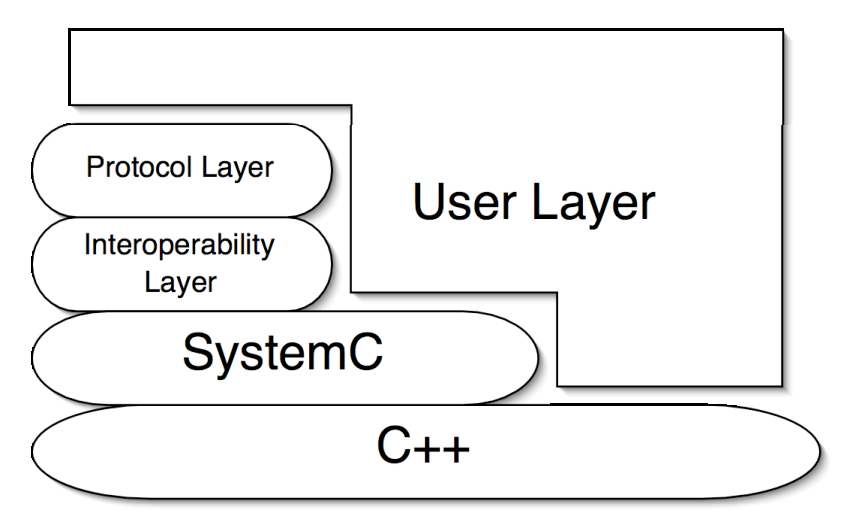
\includegraphics{SystemClayers.eps}
        \caption{SystemC Layers}
        \label{fig:layers}
\end{figure}

The User Layer will use C++, and also the SystemC library. It will
connect with the ``top'' of the protocol layer. The ``interoperability
layer'' can be hidden from the user. The interoperability interface is
implemented by the interoperability layer.  The GreenSocs
interoperability layer implements the proposed TLM WG 2.0 TLM
interoperability interface, as discussed in section~\ref{INTEROP}.

%The interoperability layer is given by two things. The API, and the data structures that must be
%transmitted across that API.  Both {\bf MUST} be used if
%interoperability is required. 

%The API is simple, it is defined by a port who's interface is an event queue that carries an
%payload. 


Another way of looking at this is from the perspective of the GreenBus
port itself. The GreenBus port is made up of a number of elements
which are designed to implement the interoperability
interface, and to provide services to the protocol
layer. Figure~\ref{fig:greenbusport} shows how these blocks
communicate.

\begin{figure}[htbp]
        \centering
        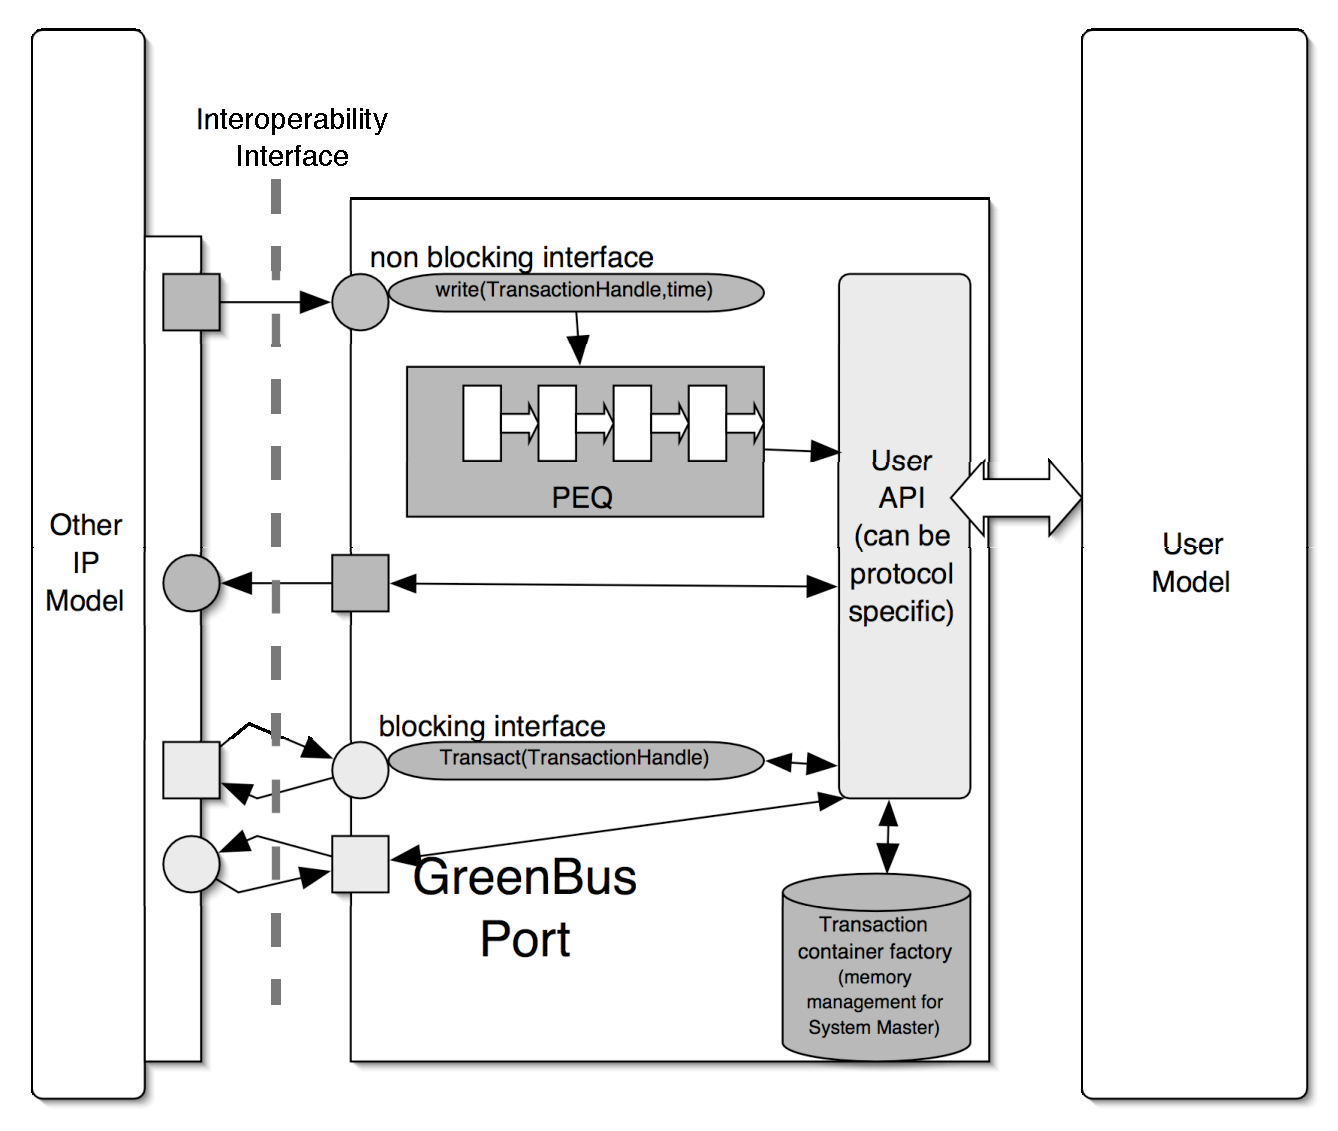
\includegraphics[scale=0.75]{GreenBusPort.eps}
        \caption{GreenBus Port}
        \label{fig:greenbusport}
\end{figure}

The PEQ is the basic component responsible for poviding the
non-blocking part of the interoperability layer. It directly
implements the ``{\tt write}'' function, and delivers the payloads to
the user model at the correct time through the ``User API''.

The transaction factory is a service provided by the GreenSocs port to
the User API to facilitate the handling of memory. It is conceptually
part of the protocol layer, but implemented as a common service as
most User API's will take advantage of it.

The User API satisfies two distinct requirements, First it defines
and operates over a specific protocol. Second, it provides the User
API that will be used to excersize the protocol.
Chapter~\ref{PROTOCOL} will describe how a protocol can be defined,
and show how the ``Generic'' protocol is defined.
Chapter~\ref{USER} will give details of the ``Generic'' protocol User API.


In Chapter~\ref{PROTOCOL}  
a list of \quarks is presented, with their SystemC implementation. The \quark
defines the semantic meaning of the information being transmitted. The SystemC
implementation is unlikely to reflect the gate-level implementation. Users are
encouraged to represent their protocols in terms of the \quarks available where
they represent the semantic meaning of the information being transmitted even if
they do not do so in the way in which their protocol would achieve the transfer
in reality.

There are 3 levels of interoperability that this system will provide

\begin{description}
\item [Full] When the same set of \quarks are used by both the protocols used in
the \master and \slave then they will be able to communicate with no adaptation.
\item [Partial] When the set of \quarks that are used by protocol are all from
within the set suggested here, then interoperability with other protocols is
likely.
\item [None] When a user defines their own \quark, there will always be the
requirement to adapt it when using IP that does not use the same protocol.
\end{description}


\section{Timing Interoperability}

As seen in Chapter~\ref{TERMS}, often protocols can be described as having a limited set of types of \atom. Just as
with the transaction data itself, the timing data must be agreed between two participants to a timed
communication. 

The mechanism chosen for timing is incredibly simply. The transaction is in a specific (timing)
state between each two participants to the communication. The state can be represented by, for
instance, an enumeration or even an integer. So long as both parties agree what data items are valid
in which state, then the communication can proceed.

The ``Generic'' protocol defined in Chapter~\ref{PROTOCOL}  has a set of data items classified in terms of which are
valid in which of the 3 \atoms (Request, Data Handshake and Response). In this way, the ``state''
variable (the {\tt phase}) identifies exactly what data is being transported when.

Because these \atoms are very generic in themselves, it is expected that most bus protocols will
simply use them, and hence interoperability at the timing level will also be achieved.
An example of this will be seen in next chapter.

\chapter{Defining a Protocol, and the Generic Protocol}
\label{PROTOCOL}

The protocol definer uses the interoperability layer and services in
the GreenBus Port to define a protocol, and
possibly define a set of user convenience functions that can be used to operate
that protocol. (It is possible that these two tasks would be carried out by
different people. The protocol owner could simply define the protocol, while
users could define their own ``convenience'' functions).
This chapter will concentrate on the definition of a protocol. The
protocol provided with GreenBus is called ``Generic''. For maximum
interoperability it should be used (or extended).

\section{ Constructing the data that is transmitted }

Firstly the protocol must be divided into the information items that are to be
transmitted. The Protocol writer is encouraged to use the \quarks provided.

More information about these \quarks can be found from OCP-IP.

\begin{tabular}{l|l|p{6.5cm}}

\multicolumn{3}{c}{Request Group} \\ \hline
 MCmd & GenericMCmdType &  Master command \\
 MAddr & unsigned long long &  Master address \\
 MAddrSpace & unsigned int &  Master address space \\
 MData & DataType & Transaction Data\\
 MDataInfo & unsigned int &  Extra information sent with the write data \\
 MByteEn & unsigned int &  Master byte enable \\
 MThreadID & unsigned int &  Master thread identifier \\
 MConnId & unsigned int &  Master connection identifier \\
 MTagID & unsigned int &  Master tag identifier  \\
 MTagInOrder & bool &  Force tag-in-order  \\
 MReqInfo & unsigned int &  Extra information sent with the response. \\
 MAtomicLength & unsigned int &  Length of atomic burst \\
 MBurstLength & unsigned int &  Burst length \\
 MBurstPrecise & bool &  Given burst length is precise \\
 MBurstSeq & GenericMBurstSeqType &  Address sequence of burst \\
 MBurstSingleReq & bool &  Burst uses single request/multiple data protocol \\
 MReqLast & bool &  Last request in a burst \\
  
\multicolumn{3}{c}{Response Group} \\ \hline
 SResp & GenericSRespType &  Slave response \\
%% SData & DataType & returned by slave \\
 SThreadI &  unsigned int &  Slave thread identifier \\
 STagID & unsigned int &  Slave tag identifier  \\
 STagInOrder & bool &  Force tag-in-order  \\
 SdataInfo & unsigned int &  Extra information sent with the response data. \\
 SrespInfo & unsigned int &  Extra information sent out with the response. \\
 SrespLast & bool &  Last response in burst \\

\multicolumn{3}{c}{Data Handshake Group} \\ \hline

 %%Mdata & DataType & The master data being sent to the slave\\
%% MdataThreadID & unsigned int &  The thread identifier for the write data \\
%5 MdataThreadI &  unsigned int & identifier for the write data \\
%% MDataTagID & unsigned int &  Data tag identifier  \\
 %%MDataByteEn & unsigned int &  The data byte enable field \\
 MDataLast & bool &  Is this the last data transfer in a burst? \\
 MDataValid & bool &  Synchronization bit. True when the master places the data
onto the channel. False after the slave has accepted the data. \\

\end{tabular}

(Note that some of the OCP attributes are not relevant as they are
already ``split'' between different phases. For TLM modeling these will
be combined into one Transaction attribute, but the phase indicator
will identify which portion of them is valid. Hence, as the phase
indicator indicates that successive Data Handshake phases have passed,
the MData field will become successively ``valid''. The way this is
done will be protocol specific, but for the ``Generic'' protocol, the
``BurstNumber'' in the Phase will indicate the byte address within the
Data array that is now the highest address with valid data in it.
% This
%point will be covered again in section ~\ref{USER_TIMING}.)

The command, response and burst types are defined as follows

\begin{verbatim}
  enum GenericMCmdType {
    Generic_MCMD_IDLE   =0,   //Idle command
    Generic_MCMD_WR     =1,   //Write command
    Generic_MCMD_RD     =2,   //Read command
    Generic_MCMD_RDEX   =3,   //Exclusive read command
    Generic_MCMD_RDL    =4,   //Read linked command
    Generic_MCMD_WRNP   =5,   //Non-posted write command
    Generic_MCMD_WRC    =6,   //Write conditional command
    Generic_MCMD_BCST   =7    //Broadcast command
  };
  
  
  enum GenericSRespType {
    Generic_SRESP_NULL =0,    //Null response
    Generic_SRESP_DVA  =1,    //Data valid/accept response
    Generic_SRESP_FAIL =2,    //Request failed
    Generic_SRESP_ERR  =3     //Error response
  };
  

  enum GenericMBurstSeqType{
    Generic_MBURSTSEQ_INCR     =0,    //Incrementing
    Generic_MBURSTSEQ_DFLT1    =1,    //Custom (packed)
    Generic_MBURSTSEQ_WRAP     =2,    //Wrapping
    Generic_MBURSTSEQ_DFLT2    =3,    //Custom (not packed)
    Generic_MBURSTSEQ_XOR      =4,    //Exclusive OR
    Generic_MBURSTSEQ_STRM     =5,    //Streaming
    Generic_MBURSTSEQ_UNKN     =6,    //Unknown
    Generic_MBURSTSEQ_RESERVED =7     //Reserved
  };

\end{verbatim}

The data and address types are slightly special.
The Address type is an unsigned 64 bit integer. Combined with the address space
\quark this is felt sufficient for the lifespan of this \quark list. Of course,
users can define their own address \quark if they need to (with the consequent
effect on interoperability). 

The data \quark is defined as a {\em pointer} to an unsigned array of bytes. This
is then wrapped into a class which will copy the data if required.
This class, and it's methods, form part of the user interface, and
will be discussed in more detail in chapter~\ref{USER}. 

So, for example, the {\em ``Generic''} protocol contains the following
\quarks :
\begin{exampleenv}
\begin{Verbatim}[ numbers=left,fontsize=\small]
  class GenericTransaction
  {
  private:
    MCmd mCmd;
    MAddr mAddr;
    MData msData;
    MBurstLength mBurstLength;
    SResp sResp;
 }
\end{Verbatim}
\end{exampleenv}

\section{ Constructing the timing points. }

For protocols that can be used to build timing models as well as purely
functional models, it is important to define the timing points of the protocol
(and the state-machine that the protocol can pass through).

The protocol must define a ``phase'' class which will be passed along with the
transaction to identify the ``state'' that the transaction is in, and therefore
which \atom is currently active, and the state progression.

This ``phase class'' is passed as a value along side all
communications, to indicate the state of the communication being
signaled (by which we mean, the state of the communication is changed), even if it occurs in the future. Therefore it is possible
to ``schedule'' a number of such communication events to indicate the
(known) progression of a transaction.
This technique is especially valuable in a so called ``passive
slave'', which only responds to input events and needs no other
methods or threads. Passive slaves are common where timing can be
statically predicted at the beginning of a transaction and will not be
affected by any other events.

For most SoC bus protocols, the 6 timing points will be sufficiently
flexible. In the {\em ``Generic''} protocol the ``phase'' is  defined thus:




\begin{exampleenv}
\begin{Verbatim}[ numbers=left,fontsize=\small]

  char phase_desc[] = "Phases for the Generic Protocol";
  class GenericPhase : public Description<phase_desc>
  {

  public:

    enum {
      Idle,
      RequestValid,RequestAccepted,
      DataValid, DataAccepted,
      ResponseValid,ResponseAccepted
    } state;

    int BurstNumber;

    GenericPhase() : state(Idle) {}

  };
\end{Verbatim}
\end{exampleenv}

Figure~\ref{fig:genericwave} shows the 3 phases of the generic
protocol, and their relationship to eachother.
Time may pass between the phases, and the bus may be used for other
transactions during this time. 

\begin{figure}[htbp]
        \centering
        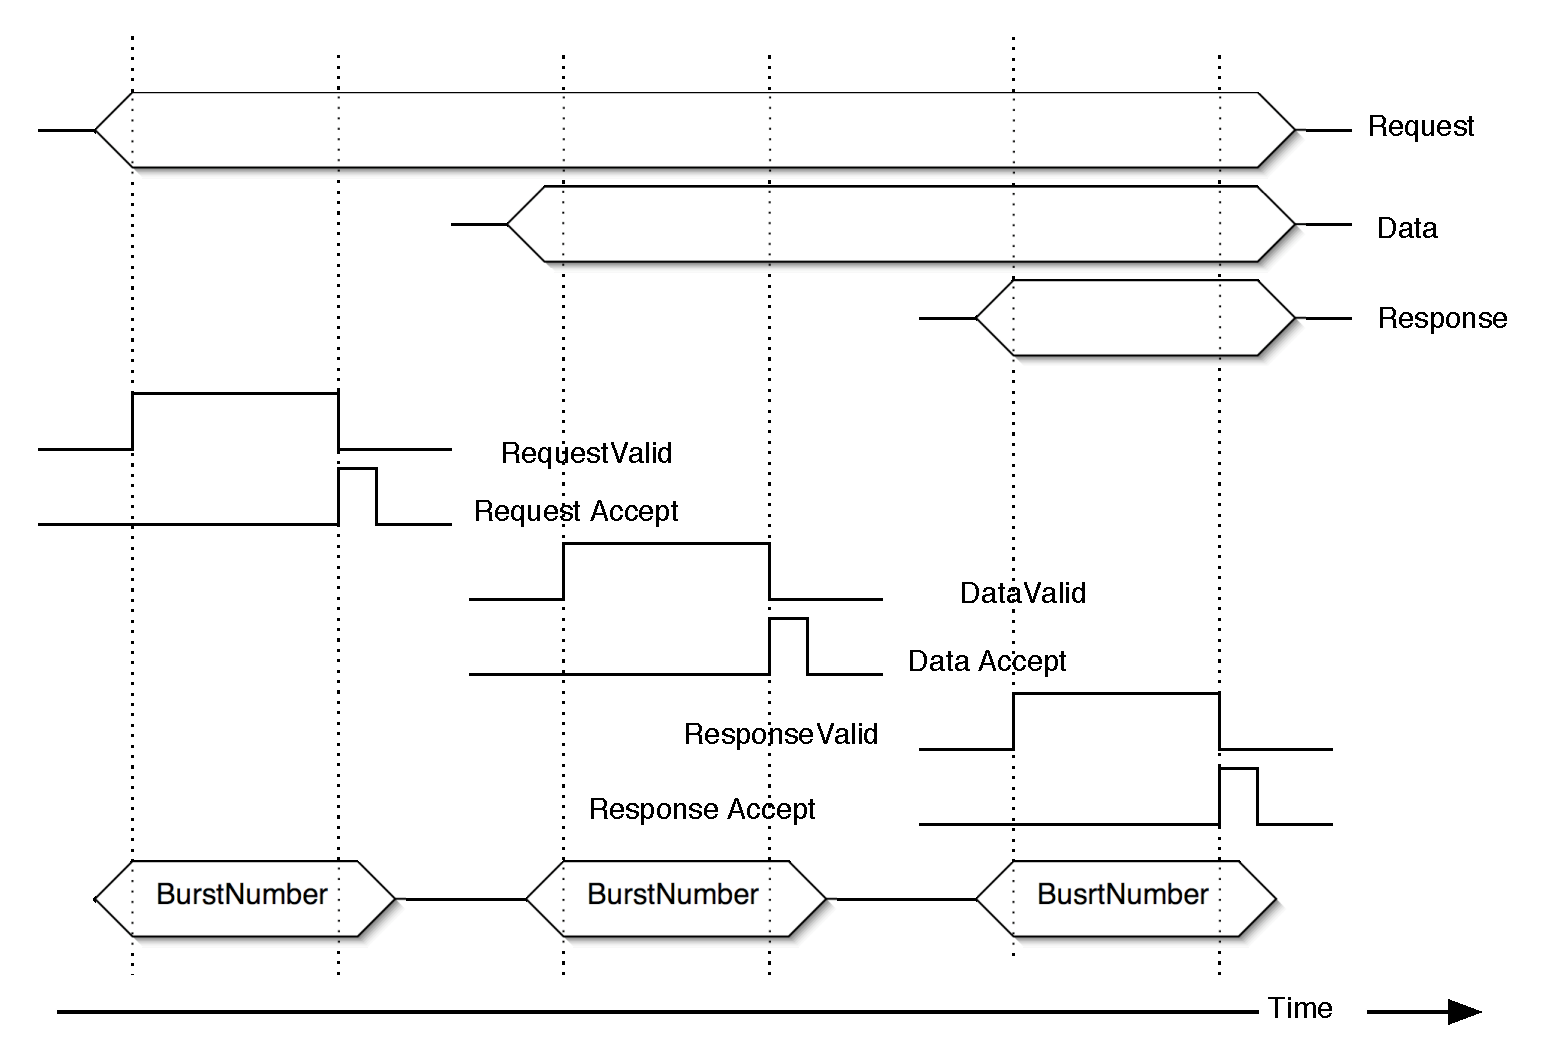
\includegraphics[scale=0.7]{GenericWaveform.eps}
        \caption{Generic Protocol Phases}
        \label{fig:genericwave}
\end{figure}

The state machine in figure~\ref{fig:genericsm} shows the state
machine for the generic protocol.

\begin{figure}[htbp]
        \centering
        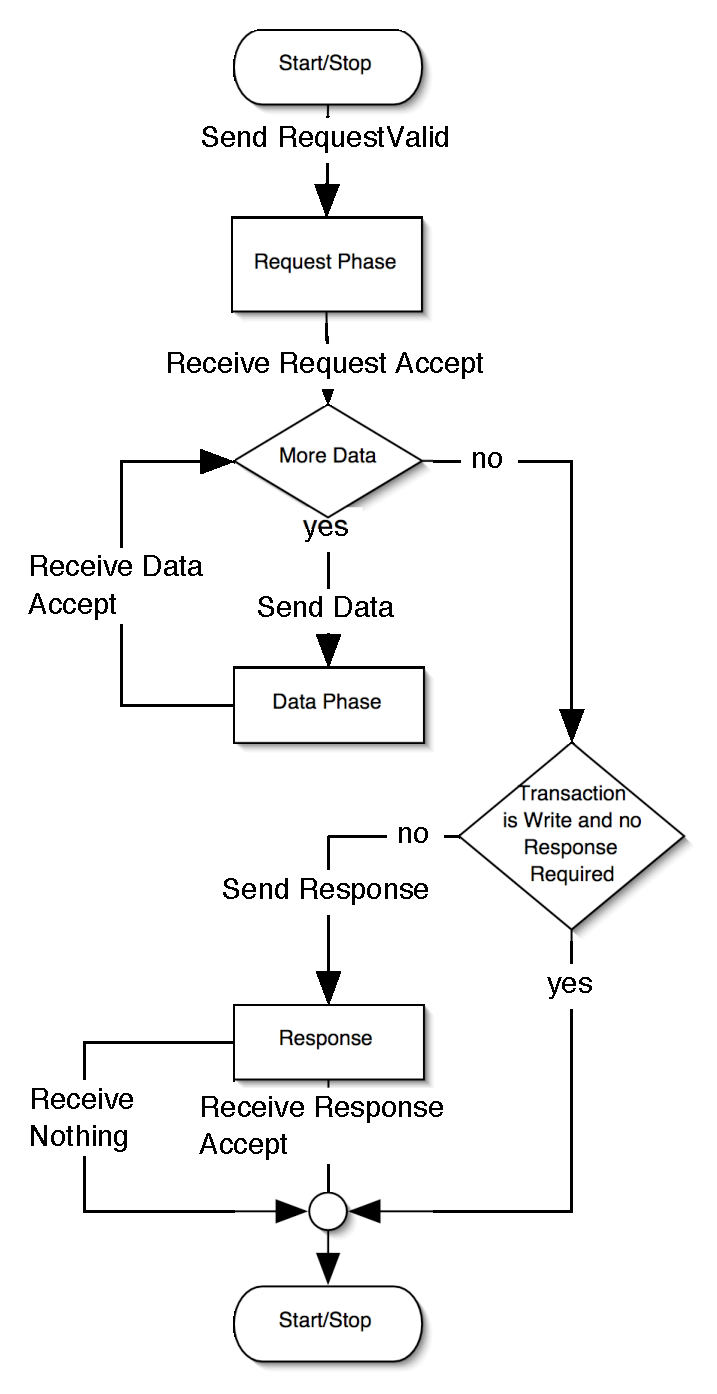
\includegraphics[scale=0.7]{GenericSM.eps}
        \caption{Generic Protocol State Machine}
        \label{fig:genericsm}
\end{figure}


The protocol makes the following important assumption: {\em Data is
accumulatively valid}. This means that once an item of data is marked
as being valid in a transaction structure, it will not be invalidated
during the lifetime transaction.  It is therefore acceptable to wait
until the end of the transaction to read the data. Equally, the entire
data payload (i.e. just the part of the transaction that carried the
data) may be written into a transaction in its entirety at the
begining of the transaction.

The {\tt RequestValid} passes from \master to \slave, and the {\tt RequestAccepted}
from \slave to \master. These signals are manditory.

It is possible to send some elements of data by setting
{\tt BurstNumber} appropriatly. The {\tt BurstNumber} gives the {\em
Byte} offset address of the higest address in which data is valid in
the transaction data field.

The {\tt DataValid} signal indicates that the data in the transaction is
valid, up to the indicated {\tt BurstNumber}. Depending on the type of
transaction (Read or Write), the DataValid will pass from \master to \slave
(Write) or from \slave to  \master (Read).

{\tt DataValid} signals may not be required (if all the data is
transmitted during either the requestor response phase).

If a {\tt DataValid} is used, then a {\tt DataAccept}  is
manditory.

Finally, a {\tt ResponseValid} passes from \slave to \master. In the case of
a read, there must be a Response, in which case the last part of the
data transfer may be in the Response. In the case of a write, the
Response is optional. In either case, the {\tt ResponseAccept} is
optional.


\subsection{Extending Generic}

Wherever possible Protocols should choose to extend the ``Generic''
protocol, rather than building an entirely new class. Since
``Generic'' is very simple, and contains only attributes which are
common to almost all busses, this is normally simple.

Care should be taken for both data and timing attributes wherever
possible that the extensions are kept optional. This will mean that IP
for the new protocol can be mixed with IP designed to be used with the
Generic protocol with no effort.

When extending a protocol, care must be taken that only attributes
which are related to data are placed in the transaction data payload,
and timing states are placed in the timing state machine. This seems
obvious, but it is not always intuitive.

Take as an example ``Split complete''. We will extend the Generic
protocol to allow a \slave to indicate to a \router that is will not
complete a transaction for some time, and the \router may use the bus
for other transactions. This will be called ``split''. When it is
ready, the \slave will indicate that it is now ready to ``complete''.

One might simply place a pair of sc\_event in the payload of the
transaction that the \slave could use to indicate things back to the
\router. While this is a workable solution, it miss-uses the
GreenBus. It adds data to the transaction payload which is, in essence
about time; also It does not use existing attributes in the transaction payload.

The solution is simply to add two extra states to the timing
protocol. The code below shows how easy this is to do. Notice that the
value of {\tt LAST\_GENERIC\_PHASE} is used to ensure that the
enumerated numbers dont overlap.

\begin{exampleenv}
\begin{Verbatim}[ numbers=left,fontsize=\small]
  namespace SplitCompletePhase
  {
    enum {
      Split = GenericPhase::LAST_GENERIC_PHASE,
      Complete
    };
  };
\end{Verbatim}
\end{exampleenv}

Now the user code may indicate a ``Split'' request, and the state
machine may pass into the ``Split'' state. Of course, a router might
simply ignore this \atom and simply maintain the bus ``locked'' to
the slave. Likewise, when the \slave is ready, it can use ``Complete''
to indicate that it can now move on. Again, a ``dumb'' router can
simply ignore this.

So, by extending the timing part of the protocol (simply adding some
additional enumerations), the data structure has remained
unchanged. Interoperability is totally unaffected. No additional data
copies are required, and no protocol conversion is necessary. All
parts of the extension are optional.

\section{ Constructing a Convenient User API }

This is the most important piece of work that must be carried out to realize a
``GreenBus''. It not only gives the user a convenient API, but should also
ensure the safe operation of the protocol.
 
To help with this, a ``basic port'' set is provided, which can be templated with
interface classes containing the user API calls that the protocol would
expect. Some examples of these are given in the generic protocol class.

The ports which are used to ``connect'' GreenBus objects together should use
shared pointers to transactions and phases. The transactions (and phases) should
be allocated inside the ports.

Notice the crucial difference between a \master port and a \router port. A
\master port must allocate memory for a transaction - it is the only
permitted object that may do so.

To assist with this memory management, ``factories'' are provided in the base
ports inside GreenBus.

Normally, protocol definers will only need to provide access classes with functions to the data
items themselves, and use the basic ports.

The next chapter will examine in detail the user API provided by the
Generic Protocol (which uses the basic port).


\chapter{Writing User Code Using the Generic Protocol}
\label{USER}

The user code will use the User API defined by the protocol writer, as
outlined in Chapter~\ref{PROTOCOL} . Therefore, the ``user code''
manual should be provided by the protocol provider.  Here we will
document the {\em ``generic''} protocol. 

\section{Basic Port}
\label{BASICPORT}

The basis of the GreenBus user interface is implemented by the
``basicport''.  Just like any SystemC  port, binding operation can be
performed. These are not documented here.

The non-blocking interface that the ``basicport'' provides is totally
based on events. An event is generated when a new {\tt PAYLOAD} is
ready to be delivered. The functions inside the ``basicport'' are
designed to provide the basic support for this. The Generic protocol
itself will define other (protocol specific) functions.

\begin{description}
\item[{\tt  void wait()}] this function simply waits for the next
{\tt PAYLOAD} to be ready on the port.

\item[{\tt  void wait()}] this function simply waits for the time that
a specific {\tt PAYLOAD} has been updated.

\item[{\tt if\_type get\_payload()}] this function returns the current
{\tt PAYLOAD}. It should only be called after an event notifying that
there is a {\tt PAYLOAD} ready.

\item[{\tt const sc\_event\& default\_event() }] this function returns an
sc\_event that can be waited on, or can be put in the sensitivity list
for a method.

\item[{\tt  transactionHandle create\_transaction()}] this function is
only available to \masters. It creates the transaction container. The
contents of the container are not guaranteed.
  
\item[{\tt   accessHandle get\_transactionHandle()}] this is a
convenience function that gets the current payload (see {\tt
get\_payload}) and extracts just the transaction data itself. The {\tt
accessHandle} is the class which provides access to the transaction
data (and is specific to the type of port - see
section~\ref{PORTCHOICE}). This function provides a safe interface to
the transaction. It should be used in preference to {\tt get\_transaction}.

\item[{\tt   phaseHandle get\_phase() }] this function provides the
handle to the phase. The phaseHandle type is defined by the
protocol. It is normally a simple class structure. In the case of the
genericbus, it simply has {\tt state} and {\tt BurstNumber} as
members.

\item[{\tt transactionHandle get\_transaction()}] this is the more
dangerous version of {\tt get\_transactionHandle()}. This function
delivers the transactionHandle directly, rather than an access class
to the transaction. From this handle it is possible to access all the
members of the transaction. This should not normally be required in a
\master or \slave, but may be useful in a verification component.

\end{description}

\section{Data Type}

The only complex attribute in the GreenBus attribute set is {\tt
mData}. It's type is defined as {\tt MasterDataType}. 

This data type carries pointers to the data, NOT the data itself. This means that data
is ``copied'' at the \slave - in that the \slave either reads the data and writes it to it's own
memory (for a write operation) or it reads from its memory and copies the results into the data
pointer (which points to memory owned by the master). In this way, the minimal number of copies is performed.

However, this means that the \master must provide an area of memory in which the transactions
data will be stored, prior to the transaction being initiated. 

The \master can only use the protocol to determine when this area of memory will be accessed, and it
is the responsibility of the \master to ensure that sufficient protocols are put in place if they
wish to share this area of memory with other threads (or indeed other interfaces).

{\tt MasterDataType} is used to store a pointer to an unsigned char
array. The array must be owned by the \master. Hence all \master data
must be ``serialized'' into an unsigned char array before it is
sent. (This can normally be achieved by a cast, if it is not
``natively'' the case.) . Be aware of endian-ness issues if your data
structure holds ``words''. If this is cast natively to an array of
unsigned chars, it will be ``host-endianed''.

{\tt MasterDataType} provides a choice of two constructors:
\begin{exampleenv}
\begin{Verbatim}[ numbers=left,fontsize=\small]
    MasterDataType()
	:size(0) {}
    MasterDataType(unsigned char *d, unsigned int s)
	:data(d),size(s){}
\end{Verbatim}
\end{exampleenv}
The copy constructor is {\tt NOT PERMITTED}, this is to prevent memory
leaks and ensure the correct use of the data type.


The unsigned char pointer in the  {\tt MasterDataType} can be set
using
\begin{exampleenv}
\begin{Verbatim}[ numbers=left,fontsize=\small]
    void set(unsigned char *d, unsigned int s){data=d;size=s;}
    void set(const MasterDataType &m){data=m.data;size=m.size;}
\end{Verbatim}
\end{exampleenv}
The first of these (line 1) takes a mandatory size argument in
addition to the pointer. It is the responsibility of the \master to
ensure that the size indicated does not exceed the size of the actual
memory allocated.

The second form ``copies'' an existing {\tt MasterDataType}. This form
can be used in place of the copy constructor. This is made explicit to
help avoid incorrect use.

{\tt MasterDataType} also provides a {\tt deepcopy}. This is used to
{\em really} copy memory between two {\tt MasterDataType}'s. 

\begin{exampleenv}
\begin{Verbatim}[ numbers=left,fontsize=\small]
    void deepcopy_to(const MasterDataType &src) {
      assert (src.size<=size);
      std::memcpy(data,src.data,src.size);
    }

    void deepcopy_from(const MasterDataType &dst) {
      assert(dst.size<=size);
      std::memcpy(dst.data,data,dst.size);
    }
\end{Verbatim}
\end{exampleenv}

Clearly these two functions should be used very sparingly. Normally
they will ONLY be used by a \slave (as the whole approach of GreenBus
is to minimize the number of data copies, and only do copies in \slaves).

Finally,  the {\tt []} operators are overloaded to give direct access
to the data, and the function {\tt byte\_size} can be used to find the
size of the {\tt MasterDataType} as given either at construction, or
during a {\tt set} function.

Here is the full code for {\tt MasterDataType}:
\begin{exampleenv}
\begin{Verbatim}[ numbers=left,fontsize=\small]
  class MasterDataType : public Description<MData_desc>{
private:
    unsigned char * data;
    unsigned int size;
public:
    MasterDataType():size(0) {}
    MasterDataType(unsigned char *d, unsigned int s)
	:data(d),size(s){}
    MasterDataType(const MasterDataType &m) {
      SC_REPORT_FATAL( 
	sc_core::SC_ID_NOT_IMPLEMENTED_, 
	"Use of copy constructor and assignment
	 operator not permitted on MasterDataType 
	(use set() instead)" );
    }
    MasterDataType &operator= (const MasterDataType &m) {
      SC_REPORT_FATAL( 
	sc_core::SC_ID_NOT_IMPLEMENTED_, 
	"Use of copy constructor and assignment
	 operator not permitted on MasterDataType
	 (use set() instead)" );
    }
    void set(unsigned char *d, unsigned int s)
	{data=d;size=s;};
    void set(const MasterDataType &m)
	{data=m.data;size=m.size;};
      
    void deepcopy_to(const MasterDataType &src) {
      assert (src.size<=size);
      std::memcpy(data,src.data,src.size);
    }

    void deepcopy_from(const MasterDataType &dst) {
      assert(dst.size<=size);
      std::memcpy(dst.data,data,dst.size);
    }

    unsigned char & operator[]  (unsigned i) 
	{assert(i<size);return data[i];}
    unsigned int byte_size(){ return size;}
  };
\end{Verbatim}
\end{exampleenv}

An example use of the {\tt MasterDataType} within a \master model
would look like this:
\begin{exampleenv}
\begin{Verbatim}[ numbers=left,fontsize=\small]
        unsigned char mem[1000];
	.
	.
	.
        t1->set_mData(MasterDataType(&mem[10],2));
\end{Verbatim}
\end{exampleenv}

The {\tt set\_mData} function call will be see later. This will
construct a new {\tt MasterDataType} ready for transmitting in a
transaction, containing just the memory in {\tt mem[10:11]}. It will
not perform any data copy, just hold a pointer to the memory.

For a \slave data copy will be needed. For the generic protocol in
GreenBus, the copy functions are handled by the user convenience layer
(which will be seen below). For instance, there is a function {\tt
get\_mData} provided, which is defined thus:
\begin{exampleenv}
\begin{Verbatim}[ numbers=left,fontsize=\small]
    void get_mData(const MData & _dst ) 
	{ msData.deepcopy_from(_dst); }
\end{Verbatim}
\end{exampleenv}

Hence the actual user code needs to have (or construct) a
{\tt MasterDataType} into, or from which to do the deep copy.
can simply. Again, this can be simply achieved as follows:
\begin{exampleenv}
\begin{Verbatim}[ numbers=left,fontsize=\small]
        unsigned char mem[1000];
	.
	.
	.
        t1->get_mData(MasterDataType( 
	& MEM[t->get_mAddr()] ,
	t->get_mBurstLength() ));
\end{Verbatim}
\end{exampleenv}

Note the use of BurstLength to determine the valid byte address. This
will always be true through the transactions lifetime. 

%The master memory type provided is shown n line 20 of the example code
%above.


\section{Port Choice}
\label{PORTCHOICE}
The user must first determine the ``type'' of the port that they wish to use for communication. This
is the ``role'' that the IP block is playing. It can be one of a \master, a \slave or a
\router. The ``port'' gives access to the transaction structures being carried between ports. 

All ports provide the functions listed in section~\ref{BASICPORT}.

A \master should use a {\tt GenericMasterPort}. This will give full write access to the request group,
and to the data handshake group for a write operation. The {\tt
GenericMasterPort} also provides one extra function which is used to
initially create a transaction. It provides a transactionHandle which
is then used by all other functions. Memory management for the
transaction is handled within the GreenBus  {\tt GenericMasterport}:
\begin{verbatim}
transactionHandle  create_transaction();
\end{verbatim}

A \slave should use a {\tt GenericSlavePort}. This will give full write access to the response group
and the data handshake group for a read operation.

A \router should use a {\tt GenericSlavePort}  to receive transaction from \masters or other \routers
and a {\tt GenericRouterPort} to send transactions to \slaves or other \routers. This will give read
access to the request group.

So, a very simple master can be built as follows:

\begin{exampleenv}
\begin{Verbatim}[numbers=left,fontsize=\small]
SC_MODULE (sillysort)
{
  GenericMasterPort init_port;
  typedef GenericMasterPort::accessHandle transactionHandle;
  typedef GenericMasterPort::phaseHandle phaseHandle;

  unsigned char mem[MEMSIZE];

  void sillysort::sendPV(transactionHandle );
  void sillysort::sendPVT(transactionHandle );
  
  sc_event ft;
  int pending;
  
  void run();
  void react();
  

  //Constructor
  SC_CTOR( sillysort ) : init_port("iport") {
    strcpy((char *)(mem),"As molt...");

    pending=0;
    
    SC_THREAD( run );

    SC_METHOD( react );
    sensitive << init_port.default_event();
    dont_initialize();

  }
};

\end{Verbatim}
\end{exampleenv}

Line 3 of this code is the critical instantiation of the generic
master port. The typedefs on lines 4 and 5 are simply for
convenience see section~\ref{TRANSACTIONHANDLE}. In this case the module will be able to perform both PV
and PVT operations, and a method is set up that will be sensitive to
the PVT timing events (lines 28, 29 and 30 set function {\tt react} up
as this method).


\section{Transaction and \atom ~ Handles}
\label{TRANSACTIONHANDLE}
All of the port access functions require a {\tt transactionHandle} and
a {\tt phaseHandle}.\\
The {\tt transactionHandle} can only be obtained from a {\tt GenericMasterPort} using the function
{\tt create\_transaction}. This should be used by the \master to create each and
every transaction. The \master should not attempt to re-use {\tt transactionHandle}s.

{\em Note: a more sophisticated protocol layer would prevent the master from re-using a
transactionHandle by recording the state of the transaction handle and ensuring that the same handle was not used in the interface functions unless it had
first been ``created''. Likewise, a more sophisticated protocol would provide a mechanism for
``caching'' pre-filled in transactions such that the master (who may issue many similar
transactions) would not need to fill them in each time. The current implementation of the Generic
protocol does not include either functionality}

Having obtained a transaction handle, a variety of interface functions are available to both read
and write to the transaction data and to process the protocol.

\section{\master ~ Port Interface}

From the \master, the access functions are:

\begin{verbatim}
 void set_mCmd(const MCmd&) 
 void set_mAddr(const MAddr&) 
 void set_mData(const MData&) 
 void set_mBurstLength(const MBurstLength&) 
 void set_mBurstSeq(const MBurstSeq&) 

 const MCmd& get_mCmd() const 
 const MAddr& get_mAddr() const 
 const MData& get_mData() const 
 const MBurstLength& get_mBurstLength() const 
 const MBurstSeq& get_mBurstSeq() const 

 const SResp& get_sResp() const 
 const SData& get_sData() const 
\end{verbatim}

Each command operates on the {\tt attribute} of the same name. See
chapter~\ref{PROTOCOL} for a full list of the attributes.  {\tt MData}
is a typedef for {\tt MasterDataType}.  Under normal circumstances,
the {\tt get\_sData} will return the same {\tt MasterDataType} as has
been set with {\tt set\_mData}. In other words, the master is
responsible for calling {\tt set\_mData} before transmitting the
transaction, {\em whether this is for a read OR a write}

It is mandatory to call all the set\_ functions before sending the
transaction.


The protocol processing functions are listed here, and will be examined
individually:

\begin{tabular}{|l|}
\hline
{\bf Blocking}\\
    {\tt void Transact(transactionHandle t)}\\
\hline
{\bf Non Blocking}\\
    {\tt void Repass(transactionHandle t, time)}\\
    {\tt void Request(transactionHandle t, time)}\\
    {\tt void SendData(transactionHandle t, time)}\\
    {\tt void AckData(transactionHandle t, time)}\\
    {\tt void AckResponse(transactionHandle t,time )}\\
\hline
\end{tabular}

{\em Note: the {\tt time} parameter above can take three forms. 
\begin{itemize}
\item It can be absent (in which case, immediate notification is
performed).
\item {\tt sc\_time}
\item {\tt double, sc\_time\_unit}
\end{itemize}}

{\em Note: a more sophisticated protocol may have functions which
combine these two ``classes'' of function (The access functions, and the protocol
processing functions) into one convenient
call. For instance {\tt read(Address, \&myData)}. The generic protocol
has been left simple so that it is obvious what is happening }

\subsection{Blocking Function: Transact}

Transact is directly implemented via the interoperability interface by
the function of the same name. A \slave {\em must} implement the
function (see below).

The Blocking function call {\tt Transact} is guaranteed to complete the transaction, though time may
pass, such that the data will be updated (or an error generated). Because time may pass, the
currently active SystemC ``process'' (i.e the sc\_thread of the \master) may yield control to other
processes, while it is waiting for the transaction to complete. One significant use of this will be
if the transaction involved accessing something which is essentially a semaphore or signaling
mechanism (often terms a synchronization point). To use the Blocking interface, the master must be
inside an sc\_thread.

\subsection{\master Non Blocking Functions}
All the other functions are non-blocking. 
It is guaranteed that a non-blocking function will return immediately, and crucially the currently
active SystemC process (in this case the \master method or thread) will not yield control. The
master can assume that data will not start returning to the master until it has finished sending
it. However, the data may come back in the same ``delta cycle'', so, sc\_signals may still have their
same state when data starts to return. If this is not the desired behavior, then the designer must
put in extra functionality to make sure that they get the effect they would like. This is a system
level synchronization issue, which should be modeled carefully.

The semantics of immediate notification (when no time is given to the
protocol processing functions) are important. All of these function
calls are non-blocking, and the user can expect them to complete with
no time passing, and no side-effects occurring that are visible to the
user. For instance, a model would not expect that a transaction would
be initiated back to the same model, from a slave, during a {\tt
Request} call. The user layer can choose to guarantee this semantic in
any way, however, the simplest approach is to schedule a SystemC style
immediate notification (which guarantees that the event will not be
processed until the current method yields).

The expectation is that the non-blocking interface will be used to
model timing effects. 

\subsubsection    {\tt void Repass(transactionHandle t, time)}
Repass simply does nothing. It can be used to keep the code consistent
when no action is required on the interface.

\subsubsection    {\tt void Request(transactionHandle t, time)}
Request signals the change in state of a transaction, to arrive in time {\tt time} using the
interoperability interface. It will set the timing state to
``RequestValid''.

\subsubsection    {\tt void SendData(transactionHandle t, time)}
SendData  signals the change in state of a transaction, to arrive in time {\tt time} using the
interoperability interface. It will set the timing state to
``DataValid''.

\subsubsection    {\tt void AckData(transactionHandle t, time)}
AckData signals the change in state of a transaction, to arrive in time {\tt time} using the
interoperability interface. It will set the timing state to
``DataAccept''.

\subsubsection    {\tt void AckResponse(transactionHandle t,time )}
AckResponse signals the change in state of a transaction, to arrive in time {\tt time} using the
interoperability interface. It will set the timing state to
``ResponseAccept''. This function is optional.


The code below is the {\tt run} method from the example module. In
this case the method performs both PV and PVT operations on the
channel.

\begin{exampleenv}
\begin{Verbatim}[numbers=left,fontsize=\small]
void sillysort::run()
{
  transactionHandle t1 = init_port.create_transaction();
  t1->set_mCmd(Generic_MCMD_WR);
  t1->set_mAddr(0x0);
  t1->set_mData(MasterDataType(&mem[0],
	strlen((char *)mem)+1));
  t1->set_mBurstLength(strlen((char *)mem)+1);
  init_port.Transact(t1);
 
  do {
    while (pending) {
       wait(ft);
    }
    
    transactionHandle t1 = init_port.create_transaction();
    t1->set_mCmd(Generic_MCMD_RD);
    t1->set_mAddr(0x0);
    t1->set_mBurstLength(strlen((char *)mem)+1);
    t1->set_mData(MasterDataType(&mem[0],
			strlen((char *)mem)+1));
    SHOW_SC_TIME(sillysort, "run: PV read from slave");
    init_port.Transact(t1);
    SHOW_SC_TIME(sillysort, "run: PV got \"" 
	<< (char *)mem << "\" from slave");

    int swaps=0;
    for (int i=0; i<strlen((char *)mem)-1; i++) {
      if (mem[i]>mem[i+1]) {
        unsigned char t=mem[i];
        mem[i]=mem[i+1];
        mem[i+1]=t;
        transactionHandle t1 = init_port.create_transaction();
        t1->set_mCmd(Generic_MCMD_WR);
        t1->set_mAddr(i);
        t1->set_mBurstLength(2);
        t1->set_mData(MasterDataType(&mem[i],2));
        SHOW_SC_TIME(sillysort, "run: start writing \"" 
	<< (char *)mem << "\" (bytes "
	<<i<<" to "<<i+1<<") to slave");
        sendPVT(t1);
        swaps++;
      }
    }
  } while (swaps);
}
\end{Verbatim}
\end{exampleenv}

Line 3 of this code requests a transaction container from the master
port. Only master ports are able to provide transaction
containers. Lines 4 to 8 fill that transaction in, and line 9 sends
the transaction as a ``PV'' transaction.

By the time the Transact function call returns, the transaction has
completed.

Lines 34 to 37 of the code set up a transaction which is used at line
41 to send a new PVT transaction. The code for sending a PVT
transaction can be very simple.

\begin{exampleenv}
\begin{Verbatim}[numbers=left,fontsize=\small]
void sillysort::sendPVT(transactionHandle t)
{
  pending++;
  
  init_port.Request(t);
  SHOW_SC_TIME(sillysort, "run: Slave Accepted."); 
}
\end{Verbatim}
\end{exampleenv}

The use of the {\tt pending} variable is to control the number of
outstanding requests that are being send to the slave. It is equally
possible that the master would carry on sending requests until the
slave indicated that it couldn't take any more - this is of course
protocol and IP dependent. Elsewhere in the code, the events generated
by the GenericMasterPort


\section{\slave ~ and \router ~ Interfaces}  

The \slave and \router should both implement the following function:
\begin{exampleenv}
\begin{Verbatim}[numbers=left,fontsize=\small]
void b_transact(GenericTransaction *);
\end{Verbatim}
\end{exampleenv}

This will then be bound to blocking {\tt Transact} interface for the
\master to use. If a \slave (or \master) does not implement this
function, a error message will be generated during run time if the
interface is called.

For both \slave and \router, the remainder of all the access functions
are non-blocking.

From the \slave, the access functions to the transaction are:

\begin{verbatim}
 void set_sResp(const SResp&) 
 void set_sData(const MData&)

 const MID& get_mID()
 const MCmd& get_mCmd()
 const MAddr& get_mAddr()
 const MData& get_mData()
 void get_mData(const MData & _dst )
 const MBurstLength& get_mBurstLength()

 const SResp& get_sResp()
 const MData& get_sData()
\end{verbatim}


From the \router, the access functions are:
\begin{verbatim}
 const MID& get_mID()
 const MCmd& get_mCmd()
 const MAddr& get_mAddr()
 const MBurstLength& get_mBurstLength()
\end{verbatim}


Each command operates on the {\tt attribute} of the same name. See
chapter~\ref{PROTOCOL} for a full list of the attributes.  {\tt MData}
is a typedef for {\tt MasterDataType}.

The case of get\_mData and set\_sData are both important:

\subsubsection{\tt virtual void set\_sData(const MData\&));}
This function does a {\em deep copy TO} the MasterDataType object
passed as a reference to the function. It should be used by a slave to
send data to the \master from it's own data structures.

\subsubsection{\tt virtual void get\_mData(const MData\&));}
This function does a {\em deep copy FROM} the MasterDataType object
passed as a reference to the function. It should be used by a slave to
copy \master data into it's own data structures.


It is mandatory to call all the set\_ functions before sending the
transaction.

For the \slave  the protocol processing functions are:

\begin{tabular}{|l|}
\hline
{\bf Blocking}\\
    Not Applicable (Slave must implement {\tt transact} )\\
\hline
{\bf Non Blocking}\\
    {\tt void Repass(transactionHandle t,time)}\\
    {\tt void Idle(transactionHandle t,time)}\\
    {\tt void FinishBlocking(transactionHandle t,time)}\\
    {\tt void SendData(transactionHandle t,time)}\\
    {\tt void AckData(transactionHandle t,time)}\\
    {\tt void Response(transactionHandle t,time)}\\
    {\tt void AckRequest(transactionHandle t,time)}\\
\hline
\end{tabular}

{\em Note: the {\tt time} parameter above can take three forms. 
\begin{itemize}
\item It can be absent (in which case, immediate notification is
performed).
\item {\tt sc\_time}
\item {\tt double, sc\_time\_unit}
\end{itemize}}

{\em Note: a more sophisticated protocol may have functions which
combine these two ``classes'' of function (The access functions, and the protocol
processing functions) into one convenient
call. For instance {\tt read(Address, \&myData)}. The generic protocol
has been left simple so that it is obvious what is happening }

The \router will use the \slave side processing functions for
communication back to the \master and the \master side processing
functions for communication onto the \slave.

Overall the \slave and \router interfaces follow much the same
mechanism as the \master interface. Because time can be given to the
protocol processing functions it
makes it possible to construct purely reactive slaves (simply an
sc\_method sensitive to its ports, which, when it receives something
instantly calculates both the response and the timing for that
response).

\subsection{\slave Non Blocking Functions}
It is guaranteed that a non-blocking function will return immediately, and crucially the currently
active SystemC process (in this case the \master method or thread) will not yield control. The
master can assume that data will not start returning to the master until it has finished sending
it. However, the data may come back in the same ``delta cycle'', so, sc\_signals may still have their
same state when data starts to return. If this is not the desired behavior, then the designer must
put in extra functionality to make sure that they get the effect they would like. This is a system
level synchronization issue, which should be modeled carefully.

The semantics of immediate notification (when no time is given to the
protocol processing functions) are important. All of these function
calls are non-blocking, and the user can expect them to complete with
no time passing, and no side-effects occurring that are visible to the
user. For instance, a model would not expect that a transaction would
be initiated back to the same model, from a slave, during a {\tt
Request} call. The user layer can choose to guarantee this semantic in
any way, however, the simplest approach is to schedule a SystemC style
immediate notification (which guarantees that the event will not be
processed until the current method yields).

The expectation is that the non-blocking interface will be used to
model timing effects. 

\subsubsection    {\tt void Repass(transactionHandle t, time)}
Repass simply does nothing. It can be used to keep the code consistent
when no action is required on the interface.


\subsubsection    {\tt void FinishBlocking(transactionHandle t, time)}
FinishBlocking signals the change in state of a transaction, (back to a \master)  to arrive in time {\tt time} using the
interoperability interface. It will set the timing state to RequestAccepted.

\subsubsection    {\tt void AckRequest(transactionHandle t, time)}
AckRequest is the same as FinishBlocking. It signals the change in state of a transaction, (back
to a \master) to arrive in time {\tt time} using the interoperability
interface. It will set the timing state to RequestAccepted.

\subsubsection    {\tt void SendData(transactionHandle t, time)}
SendData  sends  a transaction (back to a \master) to arrive in time {\tt time} using the
interoperability interface. It will set the timing state to
``DataValid''.

\subsubsection    {\tt void AckData(transactionHandle t, time)}
AckData sends  a transaction (back to a \master) to arrive in time {\tt time} using the
interoperability interface. It will set the timing state to
``DataAccept''.

\subsubsection    {\tt void Response(transactionHandle t, time)}
Response signals the change in state of a transaction, (back to a \master)  to arrive in time {\tt time} using the
interoperability interface. It will set the timing state to
``ResponseValid''.



Below is the method that is called on the receipt of an event in our
simple example. It's job is to react sensibly to all events that it
receives, and to perform all the functionality of the slave. To do so,
it will call a helper function ({\tt IPModel}) which will both perform
the required calculations and calculate the timing.

Note that some have referred to the `{\tt PVTProccess} function below
as ``the channel'' as it sits between the IP Model and the next
model. Indeed, some implementations have this process split out
completely, and use ports to connect to the {\tt IPModel} such that
different ``channels'' can be instantiated and connected.

The code below also shows how a slave can control the flow of data by
not providing a response to the initial request. This slave keeps a
number of outstanding requests active in parallel, avoiding some WAW
hazards (but not many, and only as an example, dont use this code to
design your next breaking system!)

\begin{exampleenv}
\begin{Verbatim}[numbers=left,fontsize=\small]
void simplememory::PVTProcess(GenericTargetPort::accessHandle tah,
	  GenericTargetPort::phaseHandle p){
  switch (p.state) {
    case GenericPhase::RequestValid:
      if (inWrite) {
        SHOW_SC_TIME(simplememory, 
	"PVT : can't process this write for now ");
        waiting.push_back(std::pair<
		GenericTargetPort::accessHandle,
		GenericTargetPort::phaseHandle > (tah,p));
      } else {
        target_port.FinishBlocking(tah,p,CYCLES(2) );
        if (tah->get_mCmd() == Generic_MCMD_RD) {
          target_port.SendData(tah,p,CYCLES(IPmodel(tah)));
        } else {
          inWrite=true;
        }
      }
      break;
    case GenericPhase::DataAccepted:
      if (p.BurstNumber >= tah->get_mBurstLength()) {
        target_port.Response(tah,p,CYCLES(2));
      } // we could have said "else" here, if the protocol we  
        // are trying to model sends the last item in the response
      target_port.SendData(tah,p,CYCLES(1));
      break;
    case GenericPhase::DataValid:
      if (p.BurstNumber >= tah->get_mBurstLength()) {
        SHOW_SC_TIME(simplememory, "PVT : Response send");
        target_port.Response(tah,p,CYCLES(IPmodel(tah)));
      } 
      target_port.AckData(tah,p,CYCLES(1));
      break;
    case GenericPhase::ResponseAccepted:
      SHOW_SC_TIME(simplememory, "PVT :  " << tah->get_mCmd());
      if (tah->get_mCmd() == Generic_MCMD_WR) {
        inWrite=false;
      }
      if (!inWrite) {
        if (!waiting.empty()) {
          std::pair<GenericTargetPort::accessHandle, 
	GenericTargetPort::phaseHandle > pair= waiting.front();
          waiting.pop_front();
          PVTProcess(pair.first,pair.second);
        }
      }
      break;
    default:
      SC_REPORT_ERROR( sc_core::SC_ID_INTERNAL_ERROR,''What?'');
      break;
  }
}
\end{Verbatim}
\end{exampleenv} 

The code embodies the timing functionality of the generic bus
protocol, which will be further discussed below. The critical lines
are 14 and 30 where the IP model is called in order to perform the
functionality of the slave, and to discover the (static) timing. 

The \router interface is identical to the \master interface except that no write access is given to
the data structures, and a \router port can only construct \atoms not transactions.

Care should be taken with \routers to ensure that they perform as little work as possible. Whenever
possible the same ``protocol'' should be used on all their interfaces. Sometimes, for instance in
the case of a ``bridge'' this is explicitly not the case. However, although there may be some
missing features in one bus compared to another, typically a ``bridge'' does not effect the data,
rather it effects the time taken to transmit the data.




%\section{Timing}
%\label{USER_TIMING}
%The Generic Protocol uses the basic \atoms Request, Response and Data Handshake. The convenience
%functions provided manipulate the {\tt phase} on behalf of the user. 

%The state progression for the Generic Protocol is:

%\begin{tabular}{l|l|l|}
%&{\bf Set by Master} & {\bf Set by Slave} \\
%1&Idle & \\
%2&RequestValid &\\
%3&	& RequestAccepted \\
%4&      DataValid (write) & DataValid(read)\\
% &	BurstNumber++ & BurstNumber++ \\
%5&      DataAccepted(read)	&  DataAccepted(write)\\
%6&      &ResponseValid\\
%7&	ResponseAccepted &\\
%\end{tabular}

%This protocol can be seen in the example code given above.

%The BurstNumber indicates the byte address within the Data array that is now the highest address
%with valid data in it. All bytes including and below this are assumed to be valid (the Generic
%protocol ALWAYS fills from low byte address to high byte address).

%The protocol always moves ``forward'', in that it always moves from
%Request to Data handshake to Response \atoms. However, it is
%acceptable to ``skip'' \atoms. For instance, a slave may fill in all
%the data for a read in response to a ``RequestValid'' \atom. It may
%then signal directly ``ResponseValid''.

%Transaction data is assumed to ``accumulate'' in validity. Hence, the
%``ResponseAccepted'' \atom indicates that ALL transaction data is
%valid.

%In this way, many protocols that different in terms of the quantity of
%data in a burst can communicate.

%The convenience process functions set the corresponding {\tt phase} as
%follows:

%\begin{tabular}{l|l}
%\hline
%    {\tt void Repass(transactionHandle t,time)}	& No change \\
%    {\tt void Idle(transactionHandle t,time)}		& Idle\\
%    {\tt void Request(transactionHandle t,time)}	& RequestValid\\
%    {\tt void SendData(transactionHandle t,time)}& DataValid (Burst updated)\\
%    {\tt void FinishBlocking(transactionHandle t,time)}& RequestAccepted\\
%    {\tt void AckData(transactionHandle t,time)}	& DataAccepted\\
%    {\tt void Response(transactionHandle t,time)}	& ResponseValid\\
%    {\tt void AckRequest(transactionHandle t,time)}	& RequestAccepted\\
%    {\tt void AckResponse(transactionHandle t )} & ResponseAccepted\\
%\hline
%\end{tabular}

%(FinishBlocking and AckRequest are identical in functionality, Repass
%has no functionality).

\section{Summary}

The GreenBus provides a framework in which communication fabric can be defined and efficiently
modeled. It provides enough guidance to assist in building interoperable models, while maintaining
efficiency.

For more details about GreenBus please see http://www.greensocs.com/GreenBus.
For details about the design decisions, please see http://www.greensocs.com/GreenBus/Design/


\subsection{summary of calls}

\begin{tabular}{|p{8cm}|c|c|c|}
\hline
{\bf function} & {\bf \master} & {\bf \slave}& {\bf \router} \\
 & {\bf port}  & {\bf port } & {\bf port }\\
\hline
\hline
{\bf Blocking}&&&\\
    {\tt void Transact(transactionHandle t)} & Use & Implement & Use\\
\hline
{\bf Non Blocking}&&&\\
    {\tt void Repass(transactionHandle ,time)}	& \tick & \tick & \tick \\
    {\tt void Idle(transactionHandle ,time)}		& \tick & \tick & \tick\\
    {\tt void Request(transactionHandle ,time)}	& \tick &	& \tick\\
    {\tt void SendData(transactionHandle ,time)}	& \tick & \tick & \tick\\
    {\tt void FinishBlocking(transactionHandle ,time)}& 	 & \tick &\\
    {\tt void AckData(transactionHandle ,time)}	& \tick & \tick & \tick\\
    {\tt void Response(transactionHandle ,time)}	& 	 & \tick &\\
    {\tt void AckRequest(transactionHandle ,time)}	& 	 & \tick &\\
    {\tt void AckResponse(transactionHandle ,time )} & \tick & 	& \tick\\
\hline

 {\tt void set\_mCmd(const MCmd\&) }			&\tick&&\\
 {\tt void set\_mAddr(const MAddr\&) }		&\tick&&\\
 {\tt void set\_mData(const MData\&) }			&\tick&&\\
 {\tt void set\_mBurstLength(const MBurstLength\&) }	&\tick&&\\
 {\tt void set\_mBurstSeq(const MBurstSeq\&) }		&\tick&&\\

 {\tt void set\_sResp(const SResp\&)} 			&	&\tick&\\
 {\tt void set\_sData(const MData\&)}			&	&\tick&\\

 {\tt const MCmd\& get\_mCmd()  }		&\tick&\tick&\tick\\
 {\tt const MAddr\& get\_mAddr()  }		&\tick&\tick&\tick\\
 {\tt const MData\& get\_mData()  }		&\tick&\tick&\\
 {\tt const MBurstLength\& get\_mBurstLength()  }	&\tick&\tick&\tick\\
 {\tt const MBurstSeq\& get\_mBurstSeq()  }	&\tick&&\\

 {\tt const SResp\& get\_sResp()  }		&\tick&\tick&\\
 {\tt const SData\& get\_sData()  }		&\tick&\tick&\\

 {\tt const MID\& get\_mID()}			&	&\tick&\tick\\

\hline
\end{tabular}


\appendix
\chapter{Relationship to TLM 1}

The OSCI TLM 1.0 kit has been assumed to have provided an
interoperability layer. In reality, it really provides a richer set of
functions that are more suited to supporting users code. In essence it
provides the interfaces of the protocol layer.

However, the TLM 1.0 kit did not define the semantics of the
functions, nor the data structures that were to be passed between
models. This has meant that different people have used the kit in
different ways, and in general, they have exploited a single interface
within the kit for use as part of their own interoperability layer.

Because different people have chosen different TLM 1.0 interfaces, 
different semantics, and different data structures, interoperability
has not been achieved.

The OSCI TLM 2.0 kit is proposed to have a single ``interoperability''
interface. The interoperability interface will define both
the semantics and data structures that are passed. The TLM 2.0 kit is
proposed to provide an implementation of the user layer that will
provide the TLM 1.0 interfaces.

Since many users have implemented infrastructure ``above'' the TLM 1.0
layer, they may choose to keep that infrastructure, simply using the
OSCI TLM 2.0 kit (so long as they have adhered to the same semantics
as are proposed to be used for the TLM 2.0 kit). Equally, they may
choose to re-implement their infrastructure based on the
interoperability interface.

The GreenBus infrastructure is no exception. The data structures are
those that are proposed for TLM 2.0. The underlying payload event
queue interface is the interoperability interface proposed for TLM
2.0. The user interface layer is an extension of the TLM 1.0
interfaces (specifically, for the timed interface, it uses a similar interface to the
non-blocking put, with timing added - in fact this interface is likely
to be added to the TLM 2.0 kit as well). 

GreenBus becomes one of a potentially large number of user-convenience
layers that are built on the TLM 2.0 standard interoperability
interface, with particular user interface functions and performance
characteristics. The construction of GreenBus is also ``modular''
enough to support a number of different user interfaces, so it is
perfectly possible that GreenBus would also support the TLM 1.0
interfaces - or the OCP-IP user interface.


\end{document}